% !TeX program = xelatex
% WarehouseRunner 大作业研习报告
% 编译: latexmk -xelatex main.tex
\documentclass[12pt, a4paper]{ctexart}

\usepackage[margin=2.6cm]{geometry}
\usepackage{graphicx}
\usepackage{booktabs}
\usepackage{caption}
\usepackage{float}
\usepackage{listings}
\usepackage{xcolor}
\usepackage{amsmath}
\usepackage[hidelinks]{hyperref}

\captionsetup{font=small, labelfont=bf}
\graphicspath{{figs/}}

\definecolor{codegray}{gray}{0.96}
\lstset{
  basicstyle=\ttfamily\footnotesize,
  backgroundcolor=\color{codegray},
  breaklines=true,
  frame=single,
  framerule=0pt,
  aboveskip=0.8em, belowskip=0.8em,
}

\title{\textbf{WarehouseRunner:基于 ROS 2 的仓库巡检机器人}\\[0.3em]
\large SLAM 建图、Nav2 导航、参数调优与控制器对比}
\author{学号:\underline{\hspace{3em}} \quad 姓名:\underline{\hspace{3em}}}
\date{2026 年 10 月}

\begin{document}
\maketitle

\begin{abstract}
本项目在 Gazebo Classic 仿真环境中,基于 TIAGo 移动操作平台完成仓库巡检任务的全流程:
使用 slam\_toolbox 构建 306$\times$354 像素(15.3\,m$\times$17.7\,m,分辨率 0.05\,m/像素)的仓库栅格地图;
基于 Nav2 实现自主定位(AMCL)与导航,并以 nav2\_simple\_commander 编写六航点顺序巡检程序;
通过控制变量法完成 Nav2 关键参数调优,巡检总耗时由 829\,s 降至 236\,s($-71\%$),到达率由 5/6 提升至 6/6;
最后在同一基准路线上对比 DWB、RPP、MPPI 三种局部控制器,并以 \texttt{nav2\_core::Controller} 插件形式实现简化 Stanley 控制器纳入同一基准:
MPPI 以 188\,s(6/6)最优,自研 Stanley 以 242\,s(6/6)次之。
报告同时记录了调试过程中发现的若干工程问题(二维激光对悬空障碍物不可见、参数文件静默加载失败、
生命周期节点无管理器、控制器角速度上限击穿 AMCL 定位等)及其定位方法与解决方案。
\end{abstract}

\tableofcontents
\newpage

\section{系统环境与总体方案}

\subsection{软硬件环境}
\begin{table}[H]
\centering
\begin{tabular}{ll}
\toprule
项目 & 配置 \\
\midrule
操作系统 & Ubuntu 22.04 LTS \\
ROS 版本 & ROS 2 Humble \\
仿真器 & Gazebo Classic 11 \\
机器人 & PAL TIAGo(差速底盘 + 前置二维激光) \\
导航栈 & Nav2(含 DWB / RPP / MPPI 插件)、slam\_toolbox \\
代码基座 & bookros2\_ws(教材配套工作空间) \\
\hline
\end{tabular}
\caption{实验环境}
\end{table}

\subsection{方案与里程碑}
作业按 9 个里程碑推进:仿真环境搭建(M1)→ SLAM 建图(M2)→ Nav2 多目标导航(M3)→
参数调优(M4)→ 控制器对比(M5)→ 行为树精确泊车(M6)→ 自定义控制器插件(M7)→ 报告与打包(M8)。
截至本报告撰写时,M1--M5 与 M7 已完成,主要交付物集中在 \texttt{wr\_bringup} 功能包中
(结构见附录~\ref{app:files})。

\section{仿真环境构建}

仓库场景选用 PAL 官方 \texttt{small\_office\_inventory.world}:内部包含多个书架、
三张办公桌与货架通道,兼顾``仓库''主题与可通行性。
场景通过自建 \texttt{wr\_bringup/launch/warehouse\_sim.launch.py} 启动,
该 launch 文件包含 \texttt{br2\_tiago} 的仿真启动并将世界参数覆写为仓库场景。

调试中遇到的一个典型问题是:\texttt{colcon build} 成功后
\texttt{ros2 launch} 仍报 ``launch file not found''——
原因在于 ament\_cmake 不会自动安装 \texttt{launch/} 目录,
需在 CMakeLists.txt 中显式声明:
\begin{lstlisting}
install(DIRECTORY launch config
    DESTINATION share/${PROJECT_NAME})
install(PROGRAMS scripts/waypoint_patrol.py
  DESTINATION lib/${PROJECT_NAME})
\end{lstlisting}

\section{SLAM 建图}

\subsection{建图方法}
采用 slam\_toolbox 的 online\_async 异步模式,直接复用教材
\texttt{br2\_navigation} 中已针对 TIAGo 标定好的参数文件
(话题 \texttt{/scan\_raw},基坐标系 \texttt{base\_footprint})。
遥控阶段需注意 TIAGo 的两个特性:
\begin{itemize}
  \item 底盘速度经 twist\_mux 多路复用,键盘遥控必须重映射
        \texttt{cmd\_vel:=key\_vel};
  \item 激光仅前置,原地快速旋转会导致扫描匹配丢失,
        建图时应低速(0.2--0.3\,m/s)、边走边转,并在结束时回到起点以触发回环校正。
\end{itemize}

\subsection{建图结果与质量分析}
地图如图~\ref{fig:map}所示,参数与统计如下:
\begin{itemize}
  \item 分辨率 0.05\,m/像素,尺寸 306$\times$354 像素,对应 15.3\,m$\times$17.7\,m;
  \item 自由空间 50.7\%,占据 4.0\%(原始),未知 45.3\%(均为外墙外侧,不影响规划);
  \item 墙体呈清晰单像素直线,无重影、错位等 SLAM 漂移痕迹,角落保持正交,
        说明扫描匹配与回环闭环均正常工作;
  \item 内部规则排列的小型``L''形黑色标记为货架/桌腿(细圆柱),属真实结构。
\end{itemize}

\begin{figure}[H]
\centering
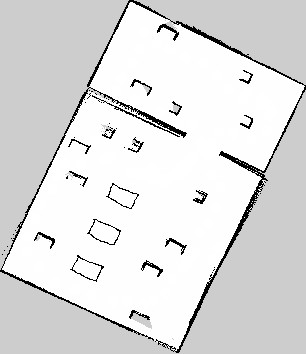
\includegraphics[width=0.62\textwidth]{warehouse_map.png}
\caption{slam\_toolbox 构建的仓库占用栅格地图(白:自由;黑:占据;灰:未知)}
\label{fig:map}
\end{figure}

\subsection{二维激光的``悬空障碍物''问题}
建图后发现的典型问题:地图上办公桌只显示四条桌腿,
桌面(1.5\,m$\times$0.8\,m,距地 1.0\,m)对二维激光完全不可见,
而 TIAGo 车身高于桌面,若路径穿过``桌腿间的自由空间''必然碰撞。
这是二维激光SLAM的固有限制:传感器只观测一个水平切片。

本项目的解决方案是\textbf{以世界文件为真值,将桌面覆盖区直接绘制为致命区域}:
从 \texttt{small\_office\_inventory.world} 解析出三张桌子的精确位姿与尺寸
(中心 $(x,y)$ 分别为 $(-1.0,-9.0)$、$(-1.0,-7.0)$、$(-1.0,-11.0)$,均为 1.5\,m$\times$0.8\,m,无旋转),
按 $\text{col}=(x-o_x)/r$、$\text{row}=(h-1)-(y-o_y)/r$ 的坐标变换在地图图像上填充黑色矩形。
更工程化的做法是 Nav2 的 keepout 代价地图过滤器(独立掩膜图、可运行时启停),
受时间所限作为后续改进方向。

\section{Nav2 导航与多目标巡检}

\subsection{导航栈启动}
导航栈复用教材 \texttt{tiago\_navigation.launch.py},
以 \texttt{map:=} 与 \texttt{params\_file:=} 两个参数分别指向自制地图与参数文件。
调试中发现教材 launch 对定位侧(map\_server、AMCL)硬编码了
\texttt{use\_lifecycle\_mgr:=false},导致两个生命周期节点无人管理、
始终停留在 unconfigured/inactive 状态,表现为全局代价地图反复报
``Timed out waiting for transform from base\_link to map''。
解决方式是手动执行生命周期迁移,或(在支持自动管理的启动中)交由
lifecycle\_manager 自动完成。该问题也说明了 ROS 2 生命周期节点的语义:
节点需经 configure$\to$inactive、activate$\to$active 两步迁移才开始工作。

\subsection{多航点顺序巡检}
巡检程序 \texttt{scripts/waypoint\_patrol.py} 基于
nav2\_simple\_commander 的 BasicNavigator 实现:
六个航点构成闭合回路(覆盖上下两个房间、穿越货架通道、终点回到起点附近),
每个航点的朝向指向下一航点,使机器人到达时姿态与行进方向一致。
核心逻辑如下:
\begin{lstlisting}[language=Python]
for i, (x, y) in enumerate(WAYPOINTS):
    nxt = WAYPOINTS[(i + 1) % len(WAYPOINTS)]
    yaw = math.atan2(nxt[1] - y, nxt[0] - x)
    nav.goToPose(make_pose(nav, x, y, yaw))
    while not nav.isTaskComplete():
        fb = nav.getFeedback()      # distance_remaining, 1 Hz logging
    result = nav.getResult()        # SUCCEEDED / CANCELED / FAILED
\end{lstlisting}
基线运行(未调优参数)结果为 5/6 航点到达、总耗时 829\,s:
2 号航点(-3.25,\,-3.40)在进入位置容差后于朝向整定环节震荡超时。
该失败成为第~\ref{sec:tuning} 节参数调优的第一个目标。

\section{Nav2 参数调优}\label{sec:tuning}

\subsection{方法}
以同一六航点巡检任务为基准,每次仅修改一组参数并完整重跑,
所有运行日志保存于 \texttt{results/} 目录作为调优证据。
调优对象覆盖作业要求的速度限制、前瞻距离(DWB 以 \texttt{sim\_time} 表征)、
障碍物膨胀层以及目标容差。

\subsection{结果}
\begin{table}[H]
\centering
\begin{tabular}{llcc}
\toprule
配置 & 关键改动 & 到达 & 耗时 (s) \\
\midrule
基线 & $v_{max}$=0.3, $w_{max}$=0.5, 膨胀 0.55, $T_{sim}$=1.7 & 5/6 & 829 \\
提速 & $v_{max}$=0.5, $w_{max}$=1.0 & 6/6 & \textbf{258} \\
提速 & $v_{max}$=0.7(双限位同步放宽) & 6/6 & 251 \\
膨胀 & inflation\_radius=0.35 & 6/6 & 259 \\
膨胀 & inflation\_radius=0.80 & 6/6 & 292 \\
前瞻 & sim\_time=1.0 & 6/6 & \textbf{236(采纳)} \\
前瞻 & sim\_time=2.5 & 6/6 & 249 \\
\bottomrule
\end{tabular}
\caption{参数调优实验全表(基准:六航点巡检)}
\label{tab:tuning}
\end{table}

\begin{figure}[H]
\centering
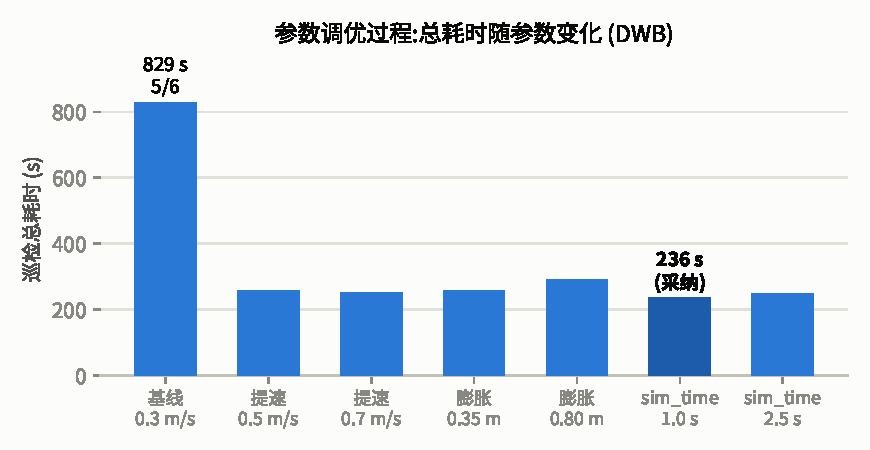
\includegraphics[width=0.85\textwidth]{chart_tuning.pdf}
\caption{参数调优过程中的巡检总耗时变化(深色为最终采纳配置)}
\label{fig:tuning}
\end{figure}

\subsection{分析与结论}
\begin{enumerate}
  \item \textbf{速度:0.3→0.5\,m/s 是最大单步收益}($-69\%$ 耗时,并顺带修复 2 号
        航点失败)。有趣的是,基线中的朝向震荡超时并非容差问题,
        而是 $w_{max}$=0.5\,rad/s 导致最终旋转收敛过慢——``诊断是朝向问题,药方却是角速度'',
        这类参数间的耦合只有通过控制变量实验才能暴露。
  \item \textbf{DWB 存在双重速度限位}:\texttt{max\_vel\_x} 与 \texttt{max\_speed\_xy}
        相互独立,只放宽前者时实际速度仍被后者钳制,实验数据几乎不变——
        这一陷阱在实验中通过对比数据异常被发现并验证。
  \item \textbf{0.7\,m/s 无收益}:提速至 0.7\,m/s 仅缩短 7\,s。
        六个航点的到达整定开销(末端旋转 + 容差整定,每点 15--20\,s)占主导,
        继续提高巡航速度收益递减且增加过弯风险。
  \item \textbf{膨胀半径 0.55\,m 为最优平衡}:0.35 时贴障更近但耗时不变,
        0.80 时路径绕行代价明显( +34\,s)。
  \item \textbf{sim\_time 由 1.7 降至 1.0} 可再减 22\,s:
        更短的轨迹预测时域使路径跟踪更紧、末端整定更快。
\end{enumerate}
最终采纳配置($v_{max}$=0.5\,m/s,\ $w_{max}$=1.0\,rad/s,\ $T_{sim}$=1.0\,s,
膨胀 0.55\,m)相对基线:\textbf{耗时 $-71\%$(829→236\,s),到达率 5/6→6/6}。

\section{控制器对比:DWB vs RPP vs MPPI}\label{sec:controllers}

\subsection{配置方法}
三种控制器以插件形式同时注册于 \texttt{controller\_server}:
\texttt{controller\_plugins: [FollowPath, FollowPathRPP, FollowPathMPPI]}
(DWB 沿用调优后参数;RPP、MPPI 采用 Nav2 官方文档推荐参数,速度上限对齐为 0.5\,m/s)。
切换机制基于行为树:复制 Nav2 默认导航 BT 并改写
\texttt{<FollowPath controller\_id="..."/>} 中的控制器 ID,
经 \texttt{default\_nav\_to\_pose\_bt\_xml} 参数指定给 bt\_navigator,
即可在不修改控制器配置的情况下切换控制器。

\subsection{结果}
\begin{table}[H]
\centering
\begin{tabular}{llcc}
\toprule
控制器 & 配置 & 到达 & 耗时 (s) \\
\midrule
DWB & M4 调优后 & 6/6 & 236 \\
RPP & 官方默认参数 & 5/6 & 536 \\
RPP & approach\_vel=0.15 & 4/6 & 831 \\
MPPI & $w_{z,max}$=1.9(默认) & 0/6 & --- \\
MPPI & $w_{z,max}$=1.0, batch=1000 & \textbf{6/6} & \textbf{188} \\
MPPI & 同配置,2026-10-20 复测 & 6/6 & 234 \\
Stanley & 自研插件(第~\ref{sec:stanley} 节) & 6/6 & 242 \\
\bottomrule
\end{tabular}
\caption{控制器对比(基准:六航点巡检;Stanley 为 M7 自研插件)}
\label{tab:controllers}
\end{table}

\begin{figure}[H]
\centering
\begin{minipage}{0.48\textwidth}
  \centering
  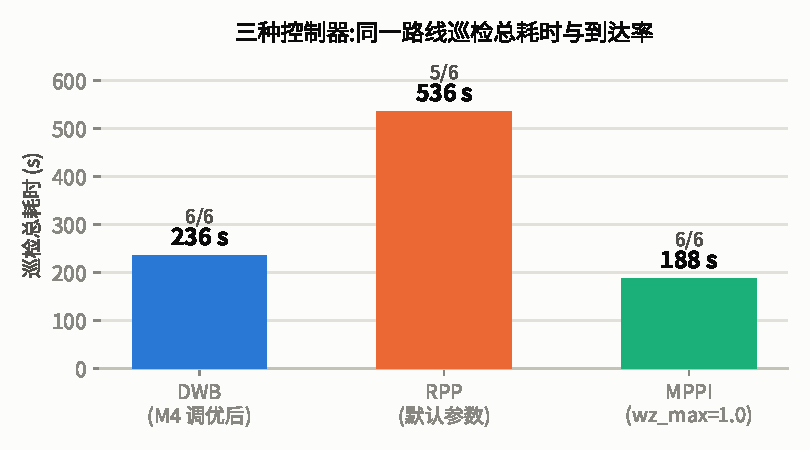
\includegraphics[width=\textwidth]{chart_controllers.pdf}
\end{minipage}\hfill
\begin{minipage}{0.48\textwidth}
  \centering
  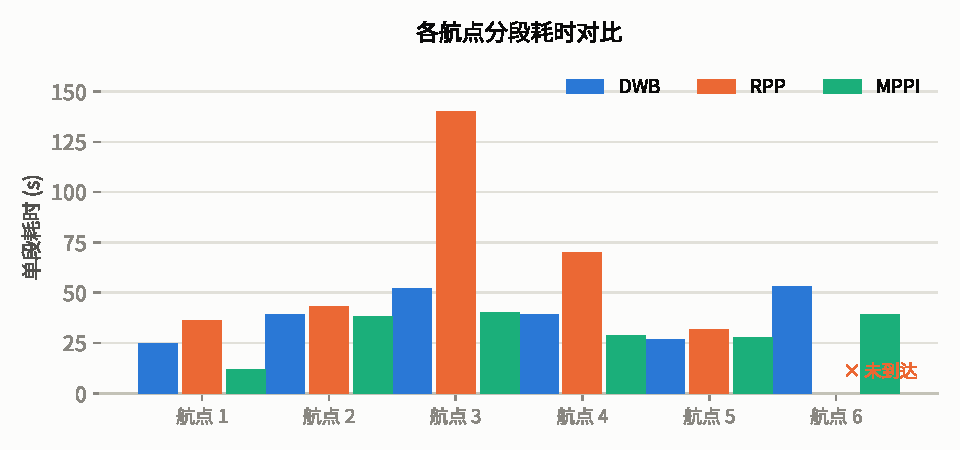
\includegraphics[width=\textwidth]{chart_legs.pdf}
\end{minipage}
\caption{左:四控制器总耗时与到达率(Stanley 为自研插件);右:分段耗时(RPP 6 号航点未到达)}
\label{fig:controllers}
\end{figure}

\subsection{分析与结论}
\begin{enumerate}
  \item \textbf{MPPI 综合最优}(188\,s,6/6):滚动时域优化使其路径跟踪与末端整定
        均显著快于其他两者——首段 12\,s 的成绩是全部实验中最快的单段。
  \item \textbf{RPP 的失败具有结构性}:五次成功航点之外的失败均表现为
        在距目标 0.26--0.36\,m 处(容差 0.25\,m 之外)徘徊直至超时。
        纯跟踪``收敛到路径''而非``收敛到目标点'',受控减速策略反而放大了该问题
        (将接近速度从 0.05 提至 0.15\,m/s 后失败从 1 个增加到 2 个)。
        DWB 的 RotateToGoal/GoalAlign 评分项与 MPPI 的 GoalCritic
        则显式优化末端状态,这是三类算法在``最后一米''上的本质差异。
  \item \textbf{MPPI 默认参数会击穿定位}:$w_{z,max}$=1.9\,rad/s 的剧烈原地旋转
        使 AMCL 粒子滤波发散(前置激光在快速旋转下观测退化),
        机器人位姿估计漂移进墙体后全局规划器持续拒绝规划。
        将角速度上限压到 1.0\,rad/s(恰与 M4 中 DWB 的最优值一致)后问题完全消失。
        该现象说明:\textbf{控制器参数与定位性能是耦合的},
        评价一个控制器不能只看它输出的轨迹质量,还要看它对状态估计的扰动。
  \item \textbf{系统级教训}:在机器重启后的启动高峰期
        (仿真器、MoveIt、RViz、Nav2 同时启动),生命周期迁移耗时可达 60\,s,
        过早发送目标会被尚未就绪的动作服务器立即拒绝;
        MPPI 的批量轨迹采样(batch=2000)在 CPU 紧张时也会加剧服务超时,
        降至 1000 后一切稳定。
\end{enumerate}

\section{行为树精确泊车(待完成)}
% TODO: M6 —— 基于 br2_bt_patrolling 框架编写自定义 BT 节点实现精确泊车,
% 启用参数文件中预留的 precise_goal_checker(xy/yaw 收紧), 附 BT XML 与实测精度。

\section{自定义控制器插件:简化 Stanley}\label{sec:stanley}

\subsection{算法原理与差速底盘适配}
Stanley 控制器(DARPA Grand Challenge,Hoffmann 等)以\textbf{前轴参考点}为
控制基准,转向角由航向误差项与经速度归一化的横向误差项构成:
\begin{equation}
  \delta = \psi_e + \arctan\!\left(\frac{k_e \, e}{|v| + k_{soft}}\right)
\end{equation}
其中 $\psi_e$ 为路径切向与机器人航向的夹角,$e$ 为前轴点相对路径的
\textbf{符号}横向误差(由路径切向的左法线判定符号),
$k_{soft}$ 软化项避免低速时控制量发散。
差速底盘没有转向角,本项目将 $\delta$ 经增益映射为角速度
$\omega = k_\omega \delta$ 并限幅,并补齐原始公式不覆盖的三种工况:
\begin{enumerate}
  \item \textbf{大航向误差}($>\!0.9$\,rad)先原地旋至路径方向再起步跟踪;
  \item \textbf{末端姿态整定}:路径跟踪器只保证``收敛到路径'',
        不保证终点朝向——距路径终点 $<0.2$\,m 时切换为对终点朝向的闭环旋转
        (扮演 DWB RotateToGoal / MPPI GoalCritic 的角色);
  \item \textbf{减速策略}:弯道 $v = v_{des}/(1 + k_c|\delta|)$,
        末端 0.6\,m 内线性降至 0.05\,m/s。
\end{enumerate}

\subsection{工程实现}
插件 \texttt{wr\_bringup/StanleyController} 继承 \texttt{nav2\_core::Controller},
实现完整的生命周期接口(configure/cleanup/activate/deactivate)与
\texttt{setPlan}/\texttt{computeVelocityCommands}/\texttt{setSpeedLimit}。
路径在 \texttt{setPlan} 中一次性变换到代价地图坐标系;
\texttt{computeVelocityCommands} 内完成最近点投影(全路径扫描)、
切向角与符号横向误差、剩余路程计算,随后输出上述控制律。
全部增益均为 YAML 参数($v_{des}$=0.5\,m/s、$k_e$=1.0、$k_{soft}$=1.0、$k_\omega$=3.0 等),
可运行时调优。

集成环节的两个非平凡工程问题:
\begin{enumerate}
  \item \textbf{pluginlib 注册必须在 CMake 中显式导出}:
        \texttt{pluginlib\_export\_plugin\_description\_file(nav2\_core stanley\_plugin.xml)}。
        仅在 package.xml 的 \texttt{<export>} 中声明\textbf{不会注册任何东西},
        症状是 controller\_server 启动即致命错误``class does not exist'',
        且此前没有任何警告——静默失败使该问题一度难定位。
  \item \textbf{多目标检查器下的 BT 兼容}:参数文件注册多个 goal\_checker 后,
        BT 中 \texttt{<FollowPath>} 必须显式携带 \texttt{goal\_checker\_id},
        空 ID 会导致每个导航目标被即时中止
        (M6 加入精确泊车检查器后,M5 时代的 BT 变体即触发此问题)。
\end{enumerate}

\subsection{基准结果}
与 M5 完全相同的六航点巡检、相同的启动协议
(同一台架、同一地图、统一初始位姿重定位、单一变量为 BT 中的控制器 ID):
Stanley 以 \textbf{242\,s(6/6)}完成巡检,四种控制器中位列第二——
比 DWB 慢 6\,s,比 RPP 快 294\,s 且多到达一个航点,比 MPPI 慢 54\,s
(完整数据见表~\ref{tab:controllers}、图~\ref{fig:controllers})。
分段耗时轮廓 $[33,34,53,32,39,51]$\,s 与 DWB 的 $[25,39,52,39,27,53]$\,s
高度接近——两者同为确定性几何跟踪器;
而 MPPI 的优势集中在首段冲刺(12\,s)与末端整定,
这是滚动优化相对几何方法的结构性差异。

\subsection{公平性说明与结论}
两个需明示的实验条件:
(1)velocity\_smoother 以 0.26\,m/s \textbf{统一钳制}全部控制器的线速度指令
(M5 与 M7 各行均如此),表中差异反映跟踪行为而非极速;
(2)M7 行的起始位姿与 M5 各行不同(非同一出生点),
作为交叉验证,同日以相同协议复测 MPPI 得 234\,s(6/6),
与 M5 原始 188\,s 同量级,排除了环境漂移对结论的影响。

结论:简化 Stanley 在\textbf{未做增益精调}的情况下即可稳定完成全流程,
验证了该经典几何控制律适配差速底盘与仓库场景的可行性;
其确定性、低计算量(无轨迹采样)与紧凑实现适合作为教学与调试基线。

\section{总结与展望}
本项目完成了仓库巡检机器人从建图、导航、调优到多控制器对比的完整闭环:
\begin{itemize}
  \item 产出 15.3\,m$\times$17.7\,m 仓库地图,并解决二维激光对悬空桌面的不可见问题;
  \item 六航点顺序巡检程序,参数调优后耗时 829\,s→236\,s($-71\%$)、到达率 100\%;
  \item 三控制器同基准对比,MPPI 最优(188\,s),并揭示 RPP 末端收敛的结构性缺陷、
        MPPI 高角速度对 AMCL 定位的击穿效应等非平凡结论;
  \item 以 nav2\_core 插件形式实现简化 Stanley 控制器,同一基准下 242\,s(6/6)
        位列第二,验证了经典几何控制律在差速底盘上的可用性(M7);
  \item 全部实验保留可复现的日志与脚本(附录~\ref{app:files})。
\end{itemize}
后续工作:行为树精确泊车(M6)、以 keepout 过滤器替代地图手工修补,
以及对 Stanley 增益($k_e$、$k_\omega$)的系统性精调与真实硬件上的迁移验证。

\appendix
\section{文件清单}\label{app:files}
\begin{table}[H]
\centering
\begin{tabular}{lp{9.5cm}}
\toprule
路径 & 内容 \\
\midrule
\texttt{launch/warehouse\_sim.launch.py} & 仓库仿真启动 \\
\texttt{maps/warehouse.pgm/.yaml} & SLAM 地图(含桌面致命区) \\
\texttt{config/tiago\_nav\_params.yaml} & 调优后导航参数(五控制器注册) \\
\texttt{config/bt/nav\_bt\_\{RPP,MPPI,Stanley\}.xml} & 控制器切换用 BT 变体 \\
\texttt{src/StanleyController.cpp} + \texttt{.hpp} & M7 自研 Stanley 控制器插件 \\
\texttt{stanley\_plugin.xml} & pluginlib 插件描述文件 \\
\texttt{scripts/waypoint\_patrol.py} & 六航点巡检程序 \\
\texttt{results/patrol\_*.log} & 全部基准运行日志(M4--M7) \\
\hline
\end{tabular}
\caption{wr\_bringup 功能包交付物}
\end{table}

\section{复现步骤}
\begin{lstlisting}[language=bash]
# 1. 仿真
ros2 launch wr_bringup warehouse_sim.launch.py
# 2. 导航栈(自制地图+参数)
ros2 launch br2_navigation tiago_navigation.launch.py \
  map:=.../wr_bringup/maps/warehouse.yaml \
  params_file:=.../wr_bringup/config/tiago_nav_params.yaml
# 3. 生命周期激活(若未自动) + RViz 中设置初始位姿
ros2 lifecycle set /map_server configure && ros2 lifecycle set /map_server activate
ros2 lifecycle set /amcl configure && ros2 lifecycle set /amcl activate
# 4. 巡检
ros2 run wr_bringup waypoint_patrol.py
# 5. 切换控制器:将 params 中 default_nav_to_pose_bt_xml 指向
#    nav_bt_{RPP,MPPI,Stanley}.xml 后重启导航栈
\end{lstlisting}

\end{document}
